\phantomsection
\definecolor{dkgreen}{rgb}{0,0.6,0}
\definecolor{gray}{rgb}{0.5,0.5,0.5}
\definecolor{mauve}{rgb}{0.58,0,0.82}

\lstset{frame=tb,
language=R,
aboveskip=3mm,
belowskip=3mm,
showstringspaces=false,
columns=flexible,
numbers=none,
inputencoding=utf8/latin1,
keywordstyle=\color{blue},
numberstyle=\tiny\color{gray},
commentstyle=\color{dkgreen},
stringstyle=\color{mauve},
breaklines=true,
breakatwhitespace=true,
tabsize=3
}

\chapter{Verifica delle ipotesi}

\section{Introduzione}

Dopo la stima dei parametri il passo successivo è la verifica delle ipotesi. La verifica delle ipotesi interviene ogni volta che si ha il bisogno di predire qualcosa, come ad esempio nelle indagini sperimentali.

In generale gli elementi che costituiscono il punto di partenza del procedimento di verifica delle ipotesi sono una popolazione descritta da una variabile aleatoria X caratterizzata da una funzione di probabilità o densità di probabilità $f(x;\theta)$, un'ipotesi su di un parametro non noto della popolazione ed un campione casuale $X_1, X_2, ..., X_n$ estratto dalla popolazione. Si può ora definire il concetto di ipotesi statistica.

\noindent \textbf{Definizione:} Un'ipotesi statistica è un'affermazione o una congettura sul parametro non noto $\theta$. Se l'ipotesi statistica specifica completamente $f(x;\theta)$ è detta ipotesi semplice, altrimenti è chiamata ipotesi composta.

\noindent \textbf{Esempio:} Sia $X_1, X_2, ..., X_n$ un campione casuale estratto da una popolazione normale con varianza nota $\delta^2$. Allora, l'ipotesi statistica $H: \mu = 1400$ è semplice poiché, essendo nota la varianza, specifica completamente la densità, mentre l'ipotesi $H: \mu \leq 1400$ è composta poiché non specifica completamente la densità. Se invece la varianza della popolazione normale non è nota, l'ipotesi statistica $H:\mu = 1400$ diventa composta poiché, essendo $\delta^2$ non nota, essa non specifica completamente la densità.

L'ipotesi soggetta a verifica viene in genere denotata con $H_0$ e viene chiamata \textbf{\textit{ipotesi nulla}}. Si chiama \textbf{test di ipotesi $\phi$} il procedimento o regola con cui si decide, sulla base dei dati del campione, se accettare o rifiutare $H_0$. La costruzione del test richiede la formulazione, in contrapposizione all'ipotesi nulla, di una proposizione alternativa. Questa proposizione prende il nome di \textbf{ipotesi alternativa} indicata con $H_1$. L'ipotesi nulla, cioè l'ipotesi soggetta a verifica, si ha quindi $\theta \in \Theta_0$ e l'ipotesi alternativa si ha quando $\theta \in \Theta_1$ e si scrive

\[H_0:\theta \in \Theta_0, \quad H_1: \theta \in \Theta_1,\]

avendo denotato con $\Theta_0$ e $\Theta_1$ due sottoinsiemi disgiunti dello spazio $\Theta$ dei parametri.

L'obiettivo è determinare un test $\phi$ che permetta di suddividere l'insieme dei campioni in due sottoinsiemi:

\begin{itemize}
    \item una regione di accettazione A,
    \item una di rifiuto R
\end{itemize}

dell'ipotesi nulla.
In generale si può incorrere in due tipi di errore

\begin{itemize}
    \item Tipo 1: rifiutare l'ipotesi nulla $H_0$ nel caso in cui tale ipotesi sia vera, denotato con 

    \[\alpha(\theta) = P(rifiutare H_0 | \theta), \quad \theta \in \Theta_0\]

    \item Tipo 2: accettare l'ipotesi nulla $H_0$ nel caso in cui tale ipotesi sia falsa, denotato con 

    \[\beta(\theta) = P(accettare H_0|\theta), \quad \theta \in \Theta_1\]
\end{itemize}

\vspace{5mm}
\begin{tabular}{c|c|c}
 & Rifiutare $H_0$ & Accettare $H_0$ \\
 $H_0$ vera & Errore del 1 tipo, probabilità $\alpha$ & Decisione esatta, probabilità $1-\alpha$ \\
 $H_0$ falsa & Decisione esatta, probabilità $1-\beta$ & Errore del 2 tipo, probabilità $\beta$
\end{tabular}
\vspace{5mm}

Un concetto importante è quello di \textbf{\textit{misura della regione critica}}.

La misura della regione critica di un test fornisce la probabilità massima di commettere un errore del 1 tipo al variare di $\theta \in \Theta_0$, ossia la probabilità massima di rifiutare l'ipotesi nulla quando essa è vera e si indica con

\[\alpha = sup_{\theta \in \Theta_0} \alpha(\theta)\]

In generale per campioni casuali di fissata ampiezza, se si diminuisce la probabilità di commettere un errore di tipo 1 aumenta la probabilità di commettere un errore di tipo 2 e viceversa. Di solito, si scelgono le ipotesi in modo da rendere l'errore di tipo 1 più grave in modo da imporre che la probabilità di commettere tale errore sia piccola. Nella costruzione del test set conviene quindi fissare la probabilità di commettere un errore di tipo 1 e cercare un test $\phi$ che minimizzi la probabilità di commettere un errore di tipo 2.

Solitamente la probabilità di commettere un errore di tipo 1 si sceglie uguale a 

\begin{itemize}
    \item 0.05, test statisticamente significativo
    \item 0.01, test statisticamente molto significativo
    \item 0.001 test statisticamente estremamente significativo
\end{itemize}

Si noti che quanto minore è il valore di $\alpha$ tanto maggiore è la credibilità di un eventuale rifiuto dell'ipotesi nulla.

I test statistici sono di due tipi: test unilaterali (detti anche unidirezionali) e test bilaterali (detti anche bidirezionali). Un test bilaterale è il seguente

\[H_0:\theta=\theta_0\]
\[H_1:\theta \neq \theta_0\]

mentre gli unilaterali sono:

\[H_0:\theta \leq \theta_0 \quad H_0:\theta \geq \theta_0\]
\[H_1:\theta > \theta_0 \quad H_1:\theta < \theta_0\]

\subsection{Test su Popolazione Normale}

In questo paragrafo si effettua la verifica delle ipotesi sul valore medio $\mu$ nel caso in cui la varianza $\delta^2$ della popolazione normale è non nota e sulla varianza $\delta^2$ nel caso in cui il valore medio $\mu$ della popolazione normale non è noto.

\vspace{5mm}
\noindent \textbf{p-value}

Nella statistica inferenziale il valore \textbf{p} (o p-value) di un test di verifica d'ipotesi indica la probabilità di ottenere un risultato uguale o "più estremo" di quello osservato, supposta vera l'ipotesi nulla. Talvolta viene anche chiamato \textbf{livello di significatività osservato}. Non dipende da $\alpha$ ma dal campione e dalla popolazione da cui è stato estratto il campione. Poiché le conclusioni dei test statistici dipendono dal livello di significatività $\alpha$, piuttosto che scegliere preventivamente un livello al quale verificare $H_0$, spesso si preferisce calcolare il p-value. Calcolando il p-value relativo ai dati osservati è possibile comportarsi come segue:

\begin{itemize}
    \item p > $\alpha$, l'ipotesi $H_0$ non può essere rifiutata;
    \item p $\leq$ $\alpha$, l'ipotesi $H_0$ deve essere rifiutata
\end{itemize}

Sia H l'ipotesi che il valore x dei dati osservati sia estratto da una certa variabile aleatoria X nota. Il p-value è definito come la probabilità, supposta l'ipotesi $H$, di ottenere un risultato (dai dati osservati) uguale o "più estremo" di quello effettivamente osservato. Il p-value è dato da:

\begin{itemize}
    \item $Pr(X \geq x|H)$ per test unilaterali destri;
    \item $Pr(X \leq x|H)$ per test unilaterali sinistri;
    \item $2 min\{Pr(X \leq x|H), Pr(X \geq x|H)\}$ per test bilaterali
\end{itemize}

\vspace{5mm}
\noindent \textbf{Test sul valore medio $\mu$ con varianza $\delta^2$ non nota}

Nelle prossime righe verrà analizzato il \textbf{test bilaterale}.

Sia $x_1, x_2, ..., x_n$ un campione casuale estratto da una popolazione normale con varianza non nota $\delta^2$. Si considerino le ipotesi:

\[H_0: \mu = \mu_0 \quad H_1:\mu \neq \mu_0\]

Essendo la varianza non nota, entrambe le ipotesi sono composte. Quando $H_0$ è vera, in analogia a quanto visto per gli intervalli di confidenza la variabile aleatoria diventa fondamentale:

\[T_n = \frac{\Bar{X}_n - \mu_0}{S_n/ \sqrt{n}}\]

che è distribuita con legge di Student con n-1 gradi di libertà. Il test bilaterale $\phi$ di misura $\alpha$ per le ipotesi $H_0$ e $H_1$ è il seguente:

\begin{itemize}
    \item si accetti $H_0$ se 
    \[-t_{\alpha/2, n-1} < \frac{\Bar{x}_n - \mu_0}{S_n/\sqrt{n}}<t_{\alpha/2, n-1}\]
    \item si rifiuti se
    \[\frac{\Bar{x}-\mu_0}{S_n/\sqrt{n}}<-t_{\alpha/2, n-1}\]

    oppure

    \[\frac{\Bar{x}-\mu_0}{S_n/\sqrt{n}}<t_{\alpha/2, n-1}\]
\end{itemize}

Si può ora applicare il test sul dataset precedentemente generato.

%test bilaterale
\vspace{5mm}
\noindent \textbf{Test statisticamente molto significativo}

Nel primo test si utilizza un livello di significatività pari all'1\%, con parametri: $H_0: \mu = 1.90$ e ipotesi alternativa $H_1: \mu \neq 1.90$. Nel caso considerato si ha dunque $\mu_0 = 1.90, \alpha = 0.01, n = 80, \Bar{x_{80}} = 1.996$ e $s_{80} = 0.510$.

\vspace{5mm}
\begin{lstlisting}
  alpha <- 0.01
  mu0 <- 1.90
  n <- length(ds)
  t_apha_m_01 <- qt(1 - alpha / 2, df = n - 1)
  t_apha_m_01
  [1] 2.639505

  meancamp <- mean(ds)
  devcamp <- sd(ds)
  t_01 <-(meancamp-mu0)/(devcamp/sqrt(n))
  t_01
  [1] 1.686455
\end{lstlisting}

\begin{figure}[!htb]
    \centering
    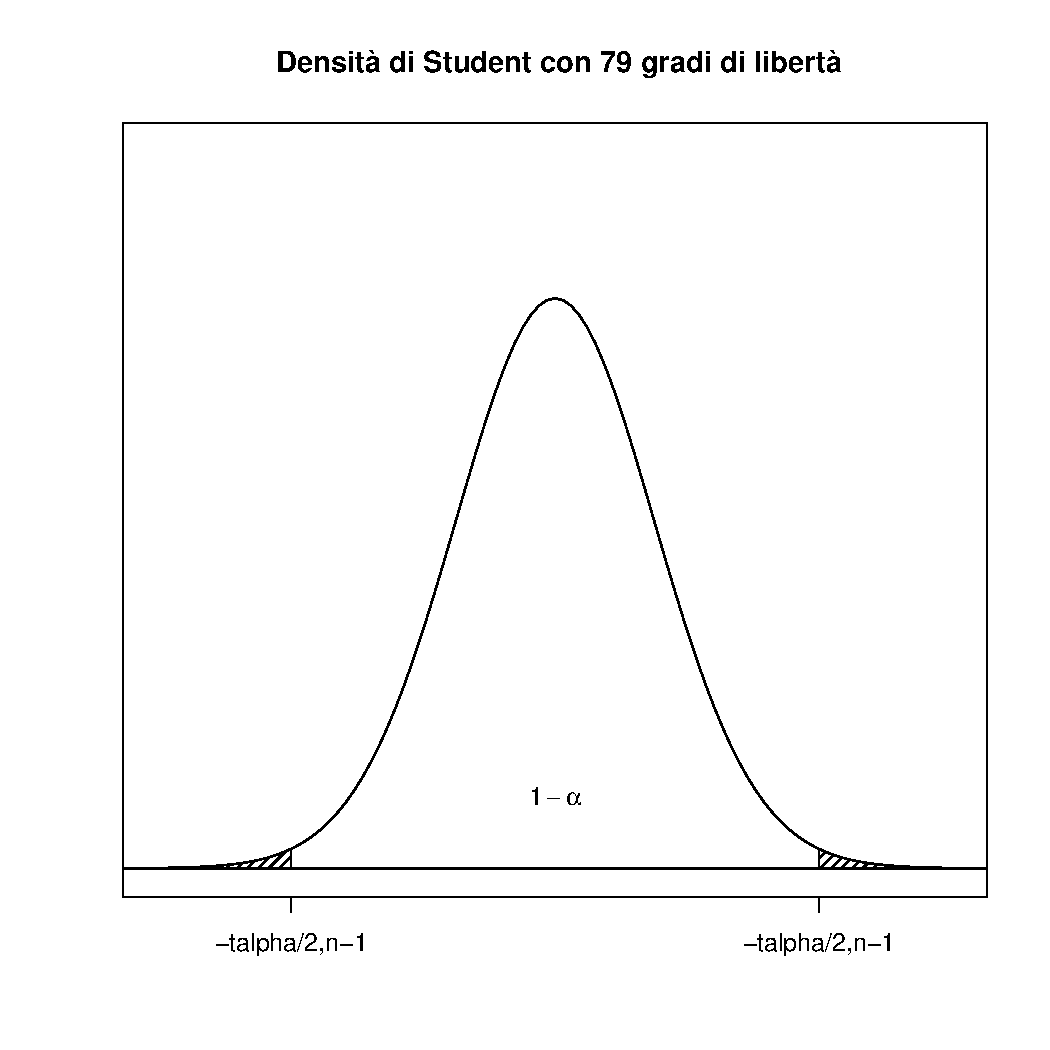
\includegraphics[height=16cm]{capitoli/images/3_verifica_ipotesi/curvehp1.pdf}
    \caption{Curva test bilaterale ipotesi 1}
\end{figure}

Dai risultati ottenuti si ha che l’ipotesi rientra nella regione di accettazione e quindi l’ipotesi $H_0$ viene accettata.

\vspace{5mm}
\noindent \textbf{Confronto con p-value}

\[pvalue = P(Z_n < -|z+{os}|) + P(Z_n > |z_{os}|) = 2P(Z_n>|z_{os}|) = 2[1-P(Z_n \leq |z_{os})],\]

\[dove \quad z_{os} = (\Bar{x}_n - \mu_0)/(\delta/\sqrt{n})\]

\begin{lstlisting}
  az <- abs(t_01)
  pvalue <- 2 * (1 - pnorm(az, mean = 0, sd = 1))
  pvalue
  [1] 0.09170812
\end{lstlisting}

Siccome $p \geq \alpha$, l'ipotesi $H_0$ viene accettata.

\vspace{5mm}
\noindent \textbf{Test statisticamente significativo}

Nel secondo test si utilizza un livello di significatività pari al 5\%, con parametri: $H_0$: $\mu = 1.90$ e ipotesi alternativa $H_1: \mu \neq 1.90$. Nel caso considerato si ha dunque $\mu_0 = 1.90, \alpha = 0.05, n = 80, \Bar{x_{80}} = 1.996$ e $s_{80} = 0.510$.

\vspace{5mm}
\begin{lstlisting}
  alpha <- 0.05
  mu0 <- 1.90
  n <- length(ds)
  t_apha_m_05 <- qt(1 - alpha / 2, df = n - 1)
  meancamp <- mean(ds)
  devcamp <- sd(ds)
  t_05 <- (meancamp - mu0) / (devcamp / sqrt(n))
  t_apha_m_05
  [1] 1.99045
  t_05
  [1] 1.686455
\end{lstlisting}

Dai risultati ottenuti si ha che l’ipotesi rientra nella regione di accettazione e quindi l’ipotesi $H_0$ viene accettata.

Nelle prossime righe si analizza il \textbf{test unilaterale sinistro}.

Sia $x_1, x_2, ..., x_n$ un campione casuale estratto da una popolazione normale con varianza non nota $\delta^2$. Si considerino le ipotesi:

\[H_0:\mu \leq \mu_0 \quad H_1:\mu > \mu_0\]

Entrambe le ipotesi $H_0$ e $H_1$ sono composte. Il test unilaterale sinistro $\psi$ di misura $\alpha$ per le ipotesi considerate è il seguente:

\begin{itemize}
    \item si accetti $H_0$ se $\frac{\Bar{x}_n - \mu_0}{s_n/\sqrt{n}} < t_{a,n-1}$
    \item si rifiuti $H_0$ se $\frac{\Bar{x}_n - \mu_0}{s_n/\sqrt{n}} > t_{a,n-1}$
\end{itemize}

Si può ora applicare il test sul dataset precedentemente generato.


%test unilaterale sinistro
\vspace{5mm}
\noindent \textbf{Test statisticamente molto significativo}

Nel primo test si utilizza un livello di significatività pari all'1\%, con parametri: $H_0$: $\mu \leq 4$ e ipotesi alternativa $H_1: \mu > 4$. Nel caso considerato si ha dunque $\mu_0 = 4, \alpha = 0.01, n = 80, \Bar{x_{80}} = 1.996$ e $s_{80} = 0.510$.

\vspace{5mm}
\begin{lstlisting}
  alpha <- 0.01
  mu0 <- 1
  n <- 80
  qt(1 - alpha, df = n - 1)
  [1] 2.374482
  
  meancamp <- mean(ds)
  devcamp <- sd(ds)
  t_01 <-(meancamp - mu0) / (devcamp / sqrt(n))
  [1] 17.44513
\end{lstlisting}

\begin{figure}[!htb]
    \centering
    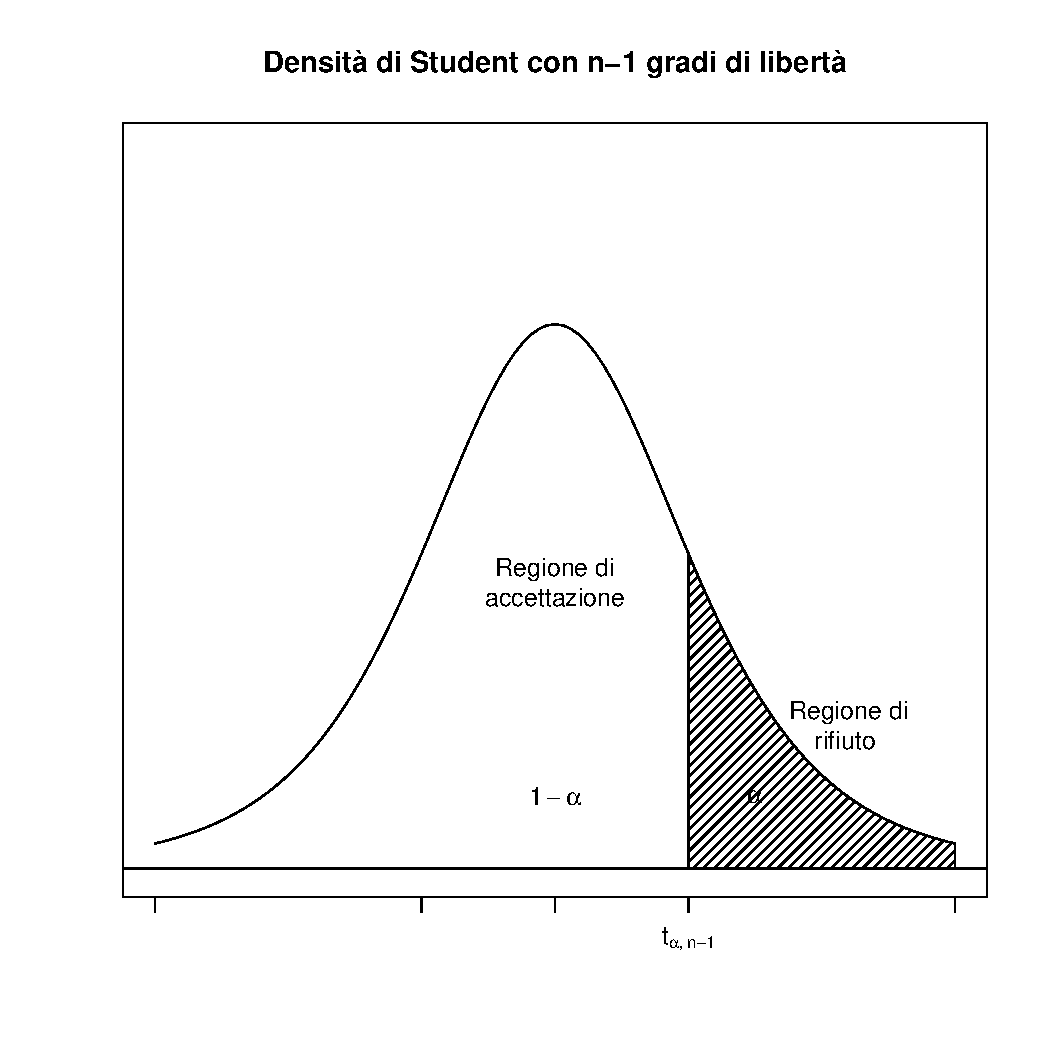
\includegraphics[height=16cm]{capitoli/images/3_verifica_ipotesi/curvehp3.pdf}
    \caption{Curva test unilaterale sinistro ipotesi 1}
\end{figure}

Dai risultati si ottiene che l'ipotesi non rientra nella regione di accettazione e quindi l'ipotesi $H_0$ viene rifiutata.

\vspace{5mm}
\noindent \textbf{Confronto con p-value}

\[pvalue = P(Z_n > z_{os}) = 1-P(Z_n \leq z_{os})\],

\[dove \quad z_{os} = (\Bar{x}_n - \mu_0)/(\delta/\sqrt{n})\]

\vspace{5mm}
\begin{lstlisting}
  z<-abs(t_01)
  pvalue <- 1 - pnorm(z, mean = 0, sd = 1)
  pvalue
  [1] 0
\end{lstlisting}

Siccome $p<\alpha$, l'ipotesi viene rifiutata.
 
\vspace{5mm}
\noindent \textbf{Test statisticamente significativo}

Nel secondo test si utilizza un livello di significatività pari al 5\%, con parametri: $H_0$: $\mu \leq 4$ e ipotesi alternativa $H_1: \mu > 4$. Nel caso considerato si ha dunque $\mu_0 = 4, \alpha = 0.05, n = 80, \Bar{x_{80}} = 1.996$ e $s_{80} = 0.510$.

\vspace{5mm}
\begin{lstlisting}
   alpha <-0.05
   mu0 <- 1
   n<- 80
   qt(1-alpha ,df=n-1)
   [1] 1.664371

   meancamp <- mean(ds)
   devcamp <- sd(ds)
   t_05 <- (meancamp - mu0) / (devcamp / sqrt(n))
   t_05
   [1] 17.44513
\end{lstlisting}

\vspace{5mm}
\begin{lstlisting}
  curve(dt(x, df = 5), from = -3, to = 3, axes = FALSE, ylim = c(0, 0.5)
    , xlab = "", ylab = "", main = "Densità di Student con n-1 gradi di libertà")
  text(0, 0.05, expression(1 - alpha))
  text(0, 0.2, "Regione di\naccettazione")
  axis(1, c(-3, -1, 0, 1, 3), c("", " ", " ", expression(t[list(alpha, n - 1)]), ""))
  vals <- seq(1, 3, length = 100)
  x <- c(1, vals, 3, 1)
  y <- c(0, dt(vals, , df = 5), 0, 0)
  polygon(x, y, density = 20, angle = 45)
  abline(h = 0)
  text(1.5, 0.05, expression(alpha))
  text(2.2, 0.1, "Regione di\nrifiuto ")
  box()
\end{lstlisting}

\begin{figure}[!htb]
    \centering
    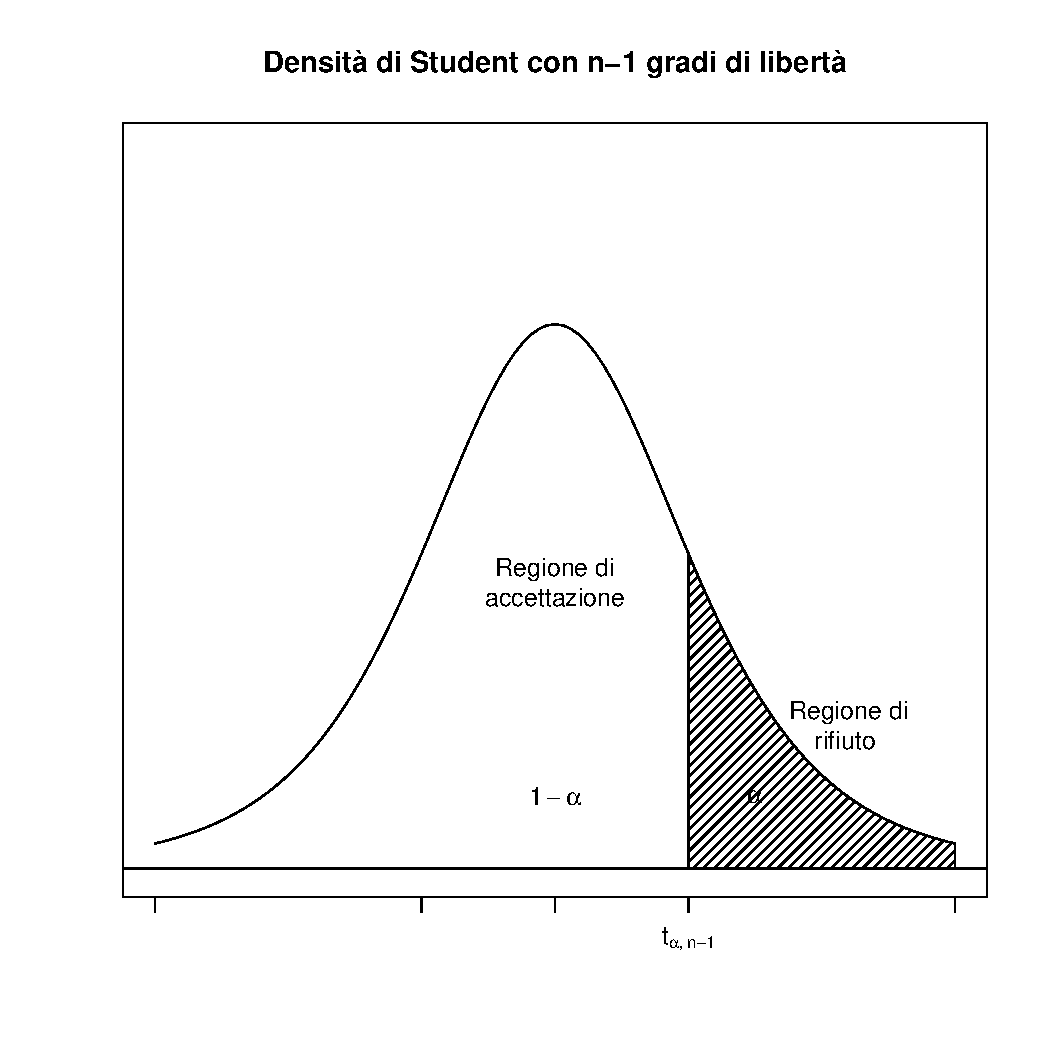
\includegraphics[height=16cm]{capitoli/images/3_verifica_ipotesi/curvehp4.pdf}
    \caption{Curva test unilaterale sinistro ipotesi 2}
\end{figure}

Dai risultati ottenuti si ha che l'ipotesi non rientra nella regione di accettazione e quindi l'ipotesi $H_0$ viene rifiutata.

Nelle prossime righe si analizza il \textbf{test unilaterale destro.}

Sia $x_1, x_2, ..., x_n$ un campione casuale estratto da una popolazione normale con varianza non nota $\delta^2$. Si considerino le ipotesi:

\[H_0:\mu \geq \mu_0 \quad H_1:\mu < \mu_0\]

Il test unilaterale destro $\psi$ di misura $\alpha$ per le ipotesi considerate è il seguente:

\begin{itemize}
    \item si accetti $H_0$ se $\frac{\Bar{x}_n - \mu_0}{s_n/\sqrt{n}} > -t_{a,n-1}$
    \item si rifiuti $H_0$ se $\frac{\Bar{x}_n - \mu_0}{s_n/\sqrt{n}} < -t_{a,n-1}$
\end{itemize}

Si può ora applicare il test sul dataset precedentemente generato

%test unilaterale destro
\vspace{5mm}
\noindent \textbf{Test statisticamente molto significativo}

Nel primo test si utilizza un livello di significatività pari all'1\%, con parametri: $H_0$: $\mu \geq 3$ e ipotesi alternativa $H_1: \mu < 3$. Nel caso considerato si ha dunque $\mu_0 = 3, \alpha = 0.01, n = 80, \Bar{x_{80}} = 1.996$ e $s_{80} = 0.510$.

\vspace{5mm}
\begin{lstlisting}
    alpha <-0.01
    mu0<-3
    n<-length(ds)
    qt(alpha ,df=n-1)
    [1] -2.374482

    meancamp <- mean(ds)
    devcamp <- sd(ds)
    t_01 <- (meancamp - mu0) / (devcamp / sqrt(n))
    t_01
    [1] -17.57414
\end{lstlisting}

\vspace{5mm}
\begin{lstlisting}
  curve(dt(x, df = n - 1), from = -3, to = 3, axes = FALSE, ylim = c(0, 0.5)
    , xlab = "", ylab = "", main = paste("Densità di Student con n-1 gradi di libertà"))
  text(0, 0.05, expression(1 - alpha))
  text(0, 0.2, "Regione di\naccettazione")
  axis(1, c(-3, -1, 0, 1, 3), c("", expression(-t[list(alpha, n - 1)]), " ", " ", ""))
  vals <- seq(-3, -1, length = 100)
  x <- c(-3, vals, -1, -3)
  y <- c(0, dt(vals, , df = 5), 0, 0)
  polygon(x, y, density = 20, angle = 45)
  abline(h = 0)
  text(-1.5, 0.05, expression(alpha))
  text(-2.2, 0.1, "Regione di\nrifiuto")
  box()
\end{lstlisting}

\begin{figure}[!htb]
    \centering
    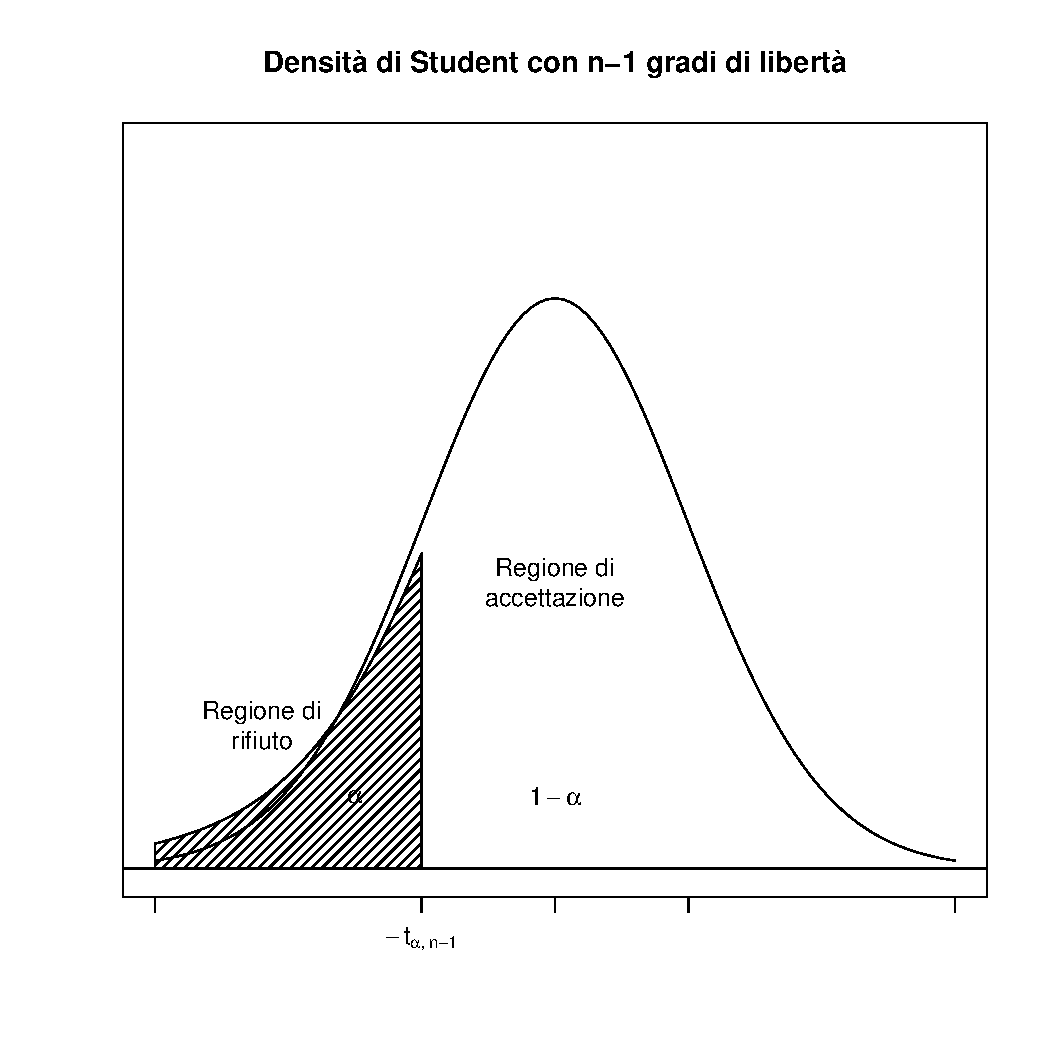
\includegraphics[height=16cm]{capitoli/images/3_verifica_ipotesi/curvehp5.pdf}
    \caption{Curva test unilaterale destro ipotesi 1}
\end{figure}

Dai risultati ottenuti si ha che l'ipotesi non rientra nella regione di accettazione e quindi l'ipotesi $H_0$ viene rifiutata.

\vspace{5mm}
\noindent \textbf{Confronto con p-value}

\[pvalue = P(Z_n \leq z_{os})\],

\[dove \quad z_{os} = (\Bar{x}_n - \mu_0)/(\delta/\sqrt{n})\]

\vspace{5mm}
\begin{lstlisting}
  z<-abs(t_01)
  pvalue <- 1 - pnorm(z, mean = 0, sd = 1)
  pvalue
  [1] 0
\end{lstlisting}

Siccome $p < \alpha$, rifiuto l'ipotesi.

\vspace{5mm}
\noindent \textbf{Test statisticamente significativo}

Nel secondo test si utilizza un livello di significatività pari al 5\%, con parametri: $H_0$: $\mu \geq 3$ e ipotesi alternativa $H_1: \mu < 3$. Nel caso considerato si ha dunque $\mu_0 = 3, \alpha = 0.05, n = 80, \Bar{x_{80}} = 1.996$ e $s_{80} = 0.510$.


\vspace{5mm}
\begin{lstlisting}
    alpha <-0.05
    mu0<-3
    n<-length(ds)
    qt(alpha ,df=n-1)
    [1] -1.664371

    meancamp <- mean(ds)
    devcamp <- sd(ds)
    t_05 <- (meancamp - mu0) / (devcamp / sqrt(n))
    t_05
    [1] -17.57414
\end{lstlisting}

\vspace{5mm}
\begin{lstlisting}
  curve(dt(x, df = n - 1), from = -3, to = 3, axes = FALSE, ylim = c(0, 0.5)
    , xlab = "", ylab = "", main = paste("Densità di Student con n-1 gradi di libertà"))
  text(0, 0.05, expression(1 - alpha))
  text(0, 0.2, "Regione di\naccettazione")
  axis(1, c(-3, -1, 0, 1, 3), c("", expression(-t[list(alpha, n - 1)]), " ", " ", ""))
  vals <- seq(-3, -1, length = 100)
  x <- c(-3, vals, -1, -3)
  y <- c(0, dt(vals, , df = 5), 0, 0)
  polygon(x, y, density = 20, angle = 45)
  abline(h = 0)
  text(-1.5, 0.05, expression(alpha))
  text(-2.2, 0.1, "Regione di\nrifiuto")
  box()
\end{lstlisting}

Dai risultati ottenuti si ha che l'ipotesi non rientra nella regione di accettazione e quindi l'ipotesi $H_0$ viene rifiutata.

\vspace{5mm}
\noindent \textbf{Test su $\delta^2$ con valore medio $\mu$ non noto}

Nelle prossime righe si analizza il \textbf{test bilaterale.}

Sia $x_1, x_2, ..., x_n$ un campione casuale estratto da una popolazione normale con valore medio non noto $\mu$. Si considerino le ipotesi:

\[H_0:\delta^2 = \delta^2_0 \quad H_0:\delta^2 \neq \delta^2_0\]

Entrambe le ipotesi sono composte. Quando l'ipotesi $H_0$ è vera, gioca un ruolo rilevante la variabile aleatoria

\[Q_n = \frac{(n-1)S_n^2}{\delta^2} = \frac{1}{\delta^2} \sum_{i=1}^n(X_i - X_n)^2\]

che è distribuita con legge chi-quadrato con n-1 gradi di libertà.

Il test bilaterale $\psi$ di misura $\alpha$ per le ipotesi considerate è:

\begin{itemize}
    \item si rifiuti $H_0$ se $\frac{(n-1)S_n^2}{\delta_0^2} < \chi_{1-\alpha/2,n-1}^2$ oppure $\frac{(n-1)S_n^2}{\delta_0^2} > \chi_{\alpha/2,n-1}^2$
    \item si accetti $H_0$ se $\chi_{1-\alpha/2,n-1}^2 < \frac{(n-1)S_n^2}{\delta_0^2} < \chi_{\alpha/2,n-1}^2$
\end{itemize}

Si può ora applicare il test sul dataset precedentemente generato.

%test bilterale
\vspace{5mm}
\noindent \textbf{Test statisticamente molto significativo}

Nel primo test si utilizza un livello di significatività pari all'1\%, con parametri: $H_0$: $\delta^2 = 1$ e ipotesi alternativa $H_1: \delta^2 \neq 1$. Nel caso considerato si ha dunque $\mu_0 = 1, \alpha = 0.01, n = 80,$ e $s_{80}^2 = 0.260$.

\vspace{5mm}
\begin{lstlisting}
  alpha <- 0.01
  sigma02 <- 1
  n <- length(ds)
  varcamp <- 0.260
  qchisq(alpha / 2, df = n - 1)
  [1] 50.37612
  qchisq(1 - alpha / 2, df = n - 1)
  [1] 115.1166
  (n-1)*varcamp /sigma02
  [1] 20.54
\end{lstlisting}

Dai risultati ottenuti si ha che l'ipotesi non rientra nella regione di accettazione e quindi l'ipotesi $H_0$ viene rifiutata.

\vspace{5mm}
\noindent \textbf{Test statisticamente significativo}

Nel secondo test si utilizza un livello di significatività pari al 5\%, con parametri: $H_0$: $\delta^2 = 1$ e ipotesi alternativa $H_1: \delta^2 \neq 1$. Nel caso considerato si ha dunque $\mu_0 = 1, \alpha = 0.05, n = 80$ e $s_{80}^2 = 0.260$.

\vspace{5mm}
\begin{lstlisting}
  alpha <- 0.05
  sigma02 <- 1
  n <- length(ds)
  varcamp <- 0.260
  qchisq(alpha / 2, df = n - 1)
  [1] 56.3089
  qchisq(1 - alpha / 2, df = n - 1)
  [1] 105.4728
  (n - 1) * varcamp / sigma02
  [1] 20.54
  
\end{lstlisting}

Dai risultati ottenuti si ha che l'ipotesi non rientra nella regione di accettazione e quindi l'ipotesi $H_0$ viene rifiutata.

Nelle prossime righe si analizza il \textbf{test unilaterale sinistro}.

Sia $x_1, x_2, ..., x_n$ un campione casuale estratto da una popolazione normale con valore medio non noto $\mu$. Si considerino le ipotesi:

\[H_0:\delta^2 \leq \delta^2_0 \quad H_0:\delta^2 > \delta^2_0\]

Entrambe le ipotesi sono composte. Quando l'ipotesi $H_0$ è vera, gioca un ruolo rilevante la variabile aleatoria

\[Q_n = \frac{(n-1)S_n^2}{\delta^2} = \frac{1}{\delta^2} \sum_{i=1}^n(X_i - X_n)^2\]

Il test bilaterale $\psi$ di misura $\alpha$ per le ipotesi considerate è: 

\begin{itemize}
    \item Si rifiuti $H_0$ se $\frac{(n-1)S_n^2}{\delta_0^2} > \chi_{\alpha/2,n-1}^2$
    \item Si accetti $H_0$ se $\frac{(n-1)S_n^2}{\delta_0^2} < \chi_{\alpha/2,n-1}^2$
\end{itemize}

Nelle prossime righe analizzeremo il \textbf{test unilaterale destro.}

Sia $x_1, x_2, ..., x_n$ un campione casuale estratto da una popolazione normale con valore medio non noto $\mu$. Si considerino le ipotesi:

\[H_0:\delta^2 \geq \delta^2_0 \quad H_0:\delta^2 < \delta^2_0\]

Entrambe le ipotesi sono composte. Quando l'ipotesi $H_0$ è vera, gioca un ruolo rilevante la variabile aleatoria

\[Q_n = \frac{(n-1)S_n^2}{\delta^2} = \frac{1}{\delta^2} \sum_{i=1}^n(X_i - X_n)^2\]

Il test bilaterale $\psi$ di misura $\alpha$ per le ipotesi considerate è: 

\begin{itemize}
    \item Si rifiuti $H_0$ se $\frac{(n-1)S_n^2}{\delta_0^2} < \chi_{1- \alpha/2,n-1}^2$
    \item Si accetti $H_0$ se $\frac{(n-1)S_n^2}{\delta_0^2} > \chi_{1- \alpha/2,n-1}^2$
\end{itemize}
%################################################

\newpage